\documentclass{report}

%%%%%%%%%%%%%%%%%%%%%%%
%       Imports       %
%%%%%%%%%%%%%%%%%%%%%%%

% Imports for document styling and formatting
\usepackage[tmargin=2cm,rmargin=1in,lmargin=1in,margin=0.85in,bmargin=2cm,footskip=.2in]{geometry} % for margins
\usepackage{xcolor} % for colors
\usepackage{bookmark} % for bookmarks
\usepackage{comment} % enables to use of multiline comments (\ifx \fi)
\usepackage{nameref} % for names
\usepackage{transparent} % for transparency
\usepackage[makeroom]{cancel} % for canceling terms
\usepackage{authblk} % for author affiliations
\usepackage{import} % for importing files
\usepackage{pdfpages} % for including pdfs
\usepackage{titletoc} % for table of contents 
\usepackage{titlesec} % For `titlecontents` and TOC customization
\usepackage{pgf} % for tikz
\usepackage[utf8]{inputenc} % for input encoding
\usepackage[T1]{fontenc} % for font encoding
\usepackage{lmodern} % for modern fonts 
\usepackage{newtxtext} % for text fonts

\setlength{\parindent}{1cm} % for paragraph indentation
\newcounter{mylabelcounter} % to create a counter for labels

\newcommand{\incfig}[1]
{
	\def\svgwidth{\columnwidth}
    \import{./figures/}{#1.pdf_tex}
} % for importing svg files
	
\usepackage{hyperref} % for hyperlinks and references

\hypersetup{
	pdftitle = {Title},
	colorlinks = true, linkcolor = doc!50!black, citecolor = doc!50!black, urlcolor = doc!50!black,
	bookmarksnumbered = true, bookmarksopen = true
} % hyperlink setup and metadata for the pdf

% Imports for Math formatting and symbols
\usepackage{amsmath, amssymb, amsthm, amsfonts, mathtools} % for math
\usepackage[varbb]{newpxmath} % for math fonts
\usepackage{xfrac} % for slanted fractions
\renewcommand\qedsymbol{$\blacksquare$} % for qed symbol

% Imports for images and diagrams 
\usepackage{graphicx} % for images

% Imports for lists, tables, columns, and boxes 
\usepackage{enumitem} % for lists
\usepackage{multicol, array} % for columns and arrays
\usepackage{varwidth} % for boxes
\usepackage[most, many, breakable]{tcolorbox} % for boxes
\tcbuselibrary{skins} % for tcolorbox libraries
\usepackage{framed} % for boxes 

% Imports for code and algorithms
\usepackage{etoolbox} % for if statements
\usepackage{xifthen} % for if statements
\usepackage[ruled,vlined,linesnumbered]{algorithm2e} % for algorithms
\SetCommentSty{mycommfont} % for comments in algorithms
\newcommand\mycommfont[1]{\footnotesize\ttfamily\textcolor{blue}{#1}} % for comments in algorithms

% Imports for references and hyperlinks
\usepackage{hyperref,theoremref} % for hyperlinks and references

% Tiks
\usepackage{tikzsymbols} % for symbols    
\usepackage{tikz} % for diagrams
\usepackage{tikz-cd} % for commutative diagrams
\usetikzlibrary{arrows,calc,shadows.blur} % for tikz libraries

\tikzset{
	symbol/.style = 
    {
			draw = none,
			every to/.append style = 
            {
					edge node = 
                    { 
                        node [sloped, allow upside down, auto = false]
                        {
                            $#1$
                        }
                    }
            }
    }
} % for symbols

%%%%%%%%%%%%%%%%%%%%%%%
%        Colors       %
%%%%%%%%%%%%%%%%%%%%%%%

\definecolor{my_red}{HTML}{bd0000} % dark red
\definecolor{my_blue}{HTML}{001589} % dark blue
\definecolor{my_green}{HTML}{033b18} % dark green
\definecolor{my_purple}{HTML}{4c0088} % dark purple
\definecolor{my_gray}{HTML}{565656} % dark gray
\definecolor{my_yellow}{HTML}{b9a900} % dark yellow 
\definecolor{my_black}{HTML}{000000} % black

\definecolor{theorem_BG}{HTML}{F2F2F9} % light gray
\definecolor{theorem_F}{HTML}{00007B} % dark blue
\definecolor{corollary_BG}{HTML}{4c0088} % dark purple
\definecolor{corollary_F}{HTML}{000000} % black
\definecolor{lemma_BG}{HTML}{196800} % dark green
\definecolor{lemma_F}{HTML}{00091e} % deep dark blue
\definecolor{proposition_BG}{HTML}{005fe8} % dark blue
\definecolor{proposition_F}{HTML}{004246} % dark teal
\definecolor{exercise_BG}{HTML}{f6fcfc} % blank white 
\definecolor{exercise_F}{HTML}{417576} % deep teal
\definecolor{example_BG}{HTML}{f9f9f9} % light gray
\definecolor{example_F}{HTML}{000000} % black
\definecolor{example_TI}{HTML}{000000} % black
\definecolor{solution_BG}{HTML}{f9f9f9} % light gray 
\definecolor{solution_F}{HTML}{000000} % black 
\definecolor{solution_TI}{HTML}{000000} % black 
\definecolor{doc}{HTML}{009fdf} % light blue
\definecolor{TOC_COLOR1}{HTML}{6000c6} % Clemson Purple
\definecolor{TOC_COLOR2}{HTML}{ffa716} % Clemson Orange

%%%%%%%%%%%%%%%%%%%%%%%
%     TCOLORBOXES     %
%%%%%%%%%%%%%%%%%%%%%%%

% The one thing that is confusing about these boxes including their names/commands
% is that they are not consistent with the actual section/chapter numbers. 
% For example, the section_theorem box is not numbered as Theorem 1.1 but as Theorem 1.1.1 
% however the chapter_theorem box is numbered as Theorem 1.1.
% In other words, section_theorem is numbered via subsection while chapter_theorem is numbered
% via section.  
% When using these commands, use chapter_box under sections and section_box under subsections.

\makeatletter
% Theorem Boxes % 
% Section Theorem 
\newtcbtheorem[number within=section]{section_theorem}{Theorem}
{
	enhanced,
	breakable,
	colback = theorem_BG,
	frame hidden,
	boxrule = 0sp,
	borderline west = {2pt}{0pt}{theorem_F},
	sharp corners,
	detach title,
	before upper = \tcbtitle\par\smallskip,
	coltitle = theorem_F,
	fonttitle = \bfseries\sffamily,
	description font = \mdseries,
	separator sign none,
	segmentation style={solid, theorem_F}
}
{theorem}

% Chapter Theorem
\newtcbtheorem[number within=chapter]{chapter_theorem}{Theorem}
{
	enhanced,
	breakable,
	colback = theorem_BG,
	frame hidden,
	boxrule = 0sp,
	borderline west = {2pt}{0pt}{theorem_F},
	sharp corners,
	detach title,
	before upper = \tcbtitle\par\smallskip,
	coltitle = theorem_F,
	fonttitle = \bfseries\sffamily,
	description font = \mdseries,
	separator sign none,
	segmentation style={solid, theorem_F}
}
{theorem}

% Corollery Boxes % 
% Section Corollary
\newtcbtheorem[number within=section]{section_corollary}{Corollary}
{
	enhanced,
	breakable,
	colback = corollary_BG!10,
	frame hidden,
	boxrule = 0sp,
	borderline west = {2pt}{0pt}{my_purple!85!corollary_F},
	sharp corners,
	detach title,
	before upper = \tcbtitle\par\smallskip,
	coltitle = corollary_BG!85!corollary_F,
	fonttitle = \bfseries\sffamily,
	description font = \mdseries,
	separator sign none,
	segmentation style={solid, corollary_BG!85!corollary_F}
}
{corollary}

% Chapter Corollary
\newtcbtheorem[number within=chapter]{chapter_corollary}{Corollary}
{
	enhanced,
	breakable,
	colback = corollary_BG!10,
	frame hidden,
	boxrule = 0sp,
	borderline west = {2pt}{0pt}{corollary_BG!85!corollary_F},
	sharp corners,
	detach title,
	before upper = \tcbtitle\par\smallskip,
	coltitle = corollary_BG!85!corollary_F,
	fonttitle = \bfseries\sffamily,
	description font = \mdseries,
	separator sign none,
	segmentation style={solid, corollary_BG!85!corollary_F}
}
{corollary}

% Lemma Boxes %
% Section Lemma
\newtcbtheorem[number within=section]{section_lemma}{Lemma}
{
	enhanced,
	breakable,
	colback = lemma_BG!10,
	frame hidden,
	boxrule = 0sp,
	borderline west = {2pt}{0pt}{lemma_F},
	sharp corners,
	detach title,
	before upper = \tcbtitle\par\smallskip,
	coltitle = lemma_F,
	fonttitle = \bfseries\sffamily,
	description font = \mdseries,
	separator sign none,
	segmentation style={solid, lemma_F}
}
{lemma}

% Chapter Lemma
\newtcbtheorem[number within=chapter]{chapter_lemma}{Lemma}
{
	enhanced,
	breakable,
	colback = lemma_BG!10,
	frame hidden,
	boxrule = 0sp,
	borderline west = {2pt}{0pt}{lemma_F},
	sharp corners,
	detach title,
	before upper = \tcbtitle\par\smallskip,
	coltitle = lemma_F,
	fonttitle = \bfseries\sffamily,
	description font = \mdseries,
	separator sign none,
	segmentation style={solid, lemma_F}
}
{lemma}

% Proposition Boxes %
% Section Proposition
\newtcbtheorem[number within=section]{section_proposition}{Proposition}
{
	enhanced,
	breakable,
	colback = proposition_BG!10,
	frame hidden,
	boxrule = 0sp,
	borderline west = {2pt}{0pt}{proposition_F},
	sharp corners,
	detach title,
	before upper = \tcbtitle\par\smallskip,
	coltitle = proposition_F,
	fonttitle = \bfseries\sffamily,
	description font = \mdseries,
	separator sign none,
	segmentation style={solid, proposition_F}
}
{proposition}

% Chapter Proposition
\newtcbtheorem[number within=chapter]{chapter_proposition}{Proposition}
{
	enhanced,
	breakable,
	colback = proposition_BG!10,
	frame hidden,
	boxrule = 0sp,
	borderline west = {2pt}{0pt}{proposition_F},
	sharp corners,
	detach title,
	before upper = \tcbtitle\par\smallskip,
	coltitle = proposition_F,
	fonttitle = \bfseries\sffamily,
	description font = \mdseries,
	separator sign none,
	segmentation style={solid, proposition_F}
}
{proposition}

% Claim Boxes %
% Section Claim 
\newtcbtheorem[number within=section]{section_claim}{Claim}
{
	enhanced,
	breakable,
	colback = my_red!10,
	frame hidden,
	boxrule = 0sp,
	borderline west = {2pt}{0pt}{my_red},
	sharp corners,
	detach title,
	before upper = \tcbtitle\par\smallskip,
	coltitle = my_red!85!my_black,
	fonttitle = \bfseries\sffamily,
	description font = \mdseries,
	separator sign none,
	segmentation style={solid, my_red!85!my_black}
}
{claim}

% Chapter Claim
\newtcbtheorem[number within=chapter]{chapter_claim}{Claim}
{
	enhanced,
	breakable,
	colback = my_red!10,
	frame hidden,
	boxrule = 0sp,
	borderline west = {2pt}{0pt}{my_red},
	sharp corners,
	detach title,
	before upper = \tcbtitle\par\smallskip,
	coltitle = my_red!85!my_black,
	fonttitle = \bfseries\sffamily,
	description font = \mdseries,
	separator sign none,
	segmentation style={solid, my_red!85!my_black}
}
{claim}

% Exercise Boxes %
% Section Exercise  
\newtcbtheorem[number within=section]{section_exercise}{Exercise}
{
	enhanced,
	breakable,
	colback = exercise_BG,
	frame hidden,
	boxrule = 0sp,
	borderline west = {2pt}{0pt}{exercise_F},
	sharp corners,
	detach title,
	before upper = \tcbtitle\par\smallskip,
	coltitle = exercise_F,
	fonttitle = \bfseries\sffamily,
	description font = \mdseries,
	separator sign none,
	segmentation style={solid, exercise_F},
}
{exercise}

% Chapter Exercise 
\newtcbtheorem[number within=chapter]{chapter_exercise}{Exercise}
{
	enhanced,
	breakable,
	colback = exercise_BG,
	frame hidden,
	boxrule = 0sp,
	borderline west = {2pt}{0pt}{exercise_F},
	sharp corners,
	detach title,
	before upper = \tcbtitle\par\smallskip,
	coltitle = exercise_F,
	fonttitle = \bfseries\sffamily,
	description font = \mdseries,
	separator sign none,
	segmentation style={solid, exercise_F},
}
{exercise}

% Example Boxes %
% Section Example 
\newtcbtheorem[number within=section]{section_example}{Example}
{
	colback = example_BG,
	breakable,
	colframe = example_F,
	coltitle = example_TI,
	boxrule = 1pt,
	sharp corners,
	detach title,
	before upper=\tcbtitle\par\smallskip,
	fonttitle = \bfseries,
	description font = \mdseries,
	separator sign none,
	description delimiters parenthesis
}
{example}

% Chapter Example
\newtcbtheorem[number within=chapter]{chapter_example}{Example}
{
	colback = example_BG,
	breakable,
	colframe = example_F,
	coltitle = example_TI,
	boxrule = 1pt,
	sharp corners,
	detach title,
	before upper=\tcbtitle\par\smallskip,
	fonttitle = \bfseries,
	description font = \mdseries,
	separator sign none,
	description delimiters parenthesis
}
{example}

% Definition Boxes %
% Section Definition
\newtcbtheorem[number within=section]{section_definition}{Definition}
{
    enhanced,
	before skip = 2mm,
    after skip = 2mm, 
    colback = red!5,
    colframe = red!80!black,
    boxrule = 0.5mm,
	attach boxed title to top left = 
    {
        xshift = 1cm,
        yshift* = 1mm-\tcboxedtitleheight,
    }, 
    varwidth boxed title* = -3cm,
	boxed title style = 
    {
        frame code = 
        {
					\path[fill = tcbcolback]
                    ([yshift = -1mm, xshift = -1mm]frame.north west)
					arc[start angle = 0, end angle = 180, radius = 1mm]
					([yshift = -1mm, xshift = 1mm]frame.north east)
					arc[start angle = 180, end angle = 0, radius = 1mm];
					\path[left color = tcbcolback!60!black, right color = tcbcolback!60!black,
						middle color = tcbcolback!80!black]
					([xshift = -2mm]frame.north west)-- 
                    ([xshift = 2mm]frame.north east)[rounded corners = 1mm]-- 
                    ([xshift = 1mm, yshift = -1mm]frame.north east)--
					(frame.south east)-- 
                    (frame.south west)--
					([xshift = -1mm, yshift = -1mm]frame.north west)[sharp corners]-- 
                    cycle;
        },
        interior engine = empty,
    },
	fonttitle = \bfseries,
	title = {#2},
    #1
}{definition}

% Chapter Definition
\newtcbtheorem[number within=chapter]{chapter_definition}{Definition}
{
    enhanced,
	before skip = 2mm,
    after skip = 2mm, 
    colback = red!5,
    colframe = red!80!black,
    boxrule = 0.5mm,
	attach boxed title to top left = 
    {
        xshift = 1cm,
        yshift* = 1mm-\tcboxedtitleheight,
    }, 
    varwidth boxed title* = -3cm,
	boxed title style = 
    {
        frame code = 
        {
					\path[fill = tcbcolback]
                    ([yshift = -1mm, xshift = -1mm]frame.north west)
					arc[start angle = 0, end angle = 180, radius = 1mm]
					([yshift = -1mm, xshift = 1mm]frame.north east)
					arc[start angle = 180, end angle = 0, radius = 1mm];
					\path[left color = tcbcolback!60!black, right color = tcbcolback!60!black,
						middle color = tcbcolback!80!black]
					([xshift = -2mm]frame.north west)-- 
                    ([xshift = 2mm]frame.north east)[rounded corners = 1mm]-- 
                    ([xshift = 1mm, yshift = -1mm]frame.north east)--
					(frame.south east)-- 
                    (frame.south west)--
					([xshift = -1mm, yshift = -1mm]frame.north west)[sharp corners]-- 
                    cycle;
        },
        interior engine = empty,
    },
	fonttitle = \bfseries,
	title = {#2},
    #1
}{definition}

% Question Boxes %
% Section Question
\newtcbtheorem[number within=section]{section_question}{Question}
{
    enhanced,
	before skip = 2mm,
    after skip = 2mm, 
    colback = my_green!5,
    colframe = my_green!80!my_black,
    boxrule = 0.5mm,
	attach boxed title to top left = 
    {
        xshift = 1cm,
        yshift* = 1mm-\tcboxedtitleheight,
    }, 
    varwidth boxed title* = -3cm,
	boxed title style = 
    {
        frame code = 
        {
					\path[fill = my_green!2!my_black]
                    ([yshift = -1mm, xshift = -1mm]frame.north west)
					arc[start angle = 0, end angle = 180, radius = 1mm]
					([yshift = -1mm, xshift = 1mm]frame.north east)
					arc[start angle = 180, end angle = 0, radius = 1mm];
					\path[left color = my_green!60!black, right color = my_green!60!black,
						middle color = my_green!80!black]
					([xshift = -2mm]frame.north west)-- 
                    ([xshift = 2mm]frame.north east)[rounded corners = 1mm]-- 
                    ([xshift = 1mm, yshift = -1mm]frame.north east)--
					(frame.south east)-- 
                    (frame.south west)--
					([xshift = -1mm, yshift = -1mm]frame.north west)[sharp corners]-- 
                    cycle;
        },
        interior engine = empty,
    },
	fonttitle = \bfseries,
	title = {#2},
    #1
}{question}

% Chapter Question 
\newtcbtheorem[number within=chapter]{chapter_question}{Question}
{
    enhanced,
	before skip = 2mm,
    after skip = 2mm, 
    colback = my_green!5,
    colframe = my_green!80!my_black,
    boxrule = 0.5mm,
	attach boxed title to top left = 
    {
        xshift = 1cm,
        yshift* = 1mm-\tcboxedtitleheight,
    }, 
    varwidth boxed title* = -3cm,
	boxed title style = 
    {
        frame code = 
        {
					\path[fill = my_green!2!my_black]
                    ([yshift = -1mm, xshift = -1mm]frame.north west)
					arc[start angle = 0, end angle = 180, radius = 1mm]
					([yshift = -1mm, xshift = 1mm]frame.north east)
					arc[start angle = 180, end angle = 0, radius = 1mm];
					\path[left color = my_green!60!black, right color = my_green!60!black,
						middle color = my_green!80!black]
					([xshift = -2mm]frame.north west)-- 
                    ([xshift = 2mm]frame.north east)[rounded corners = 1mm]-- 
                    ([xshift = 1mm, yshift = -1mm]frame.north east)--
					(frame.south east)-- 
                    (frame.south west)--
					([xshift = -1mm, yshift = -1mm]frame.north west)[sharp corners]-- 
                    cycle;
        },
        interior engine = empty,
    },
	fonttitle = \bfseries,
	title = {#2},
    #1
}{question}

% Solution Boxes % 
% Section Solution
\newtcbtheorem[number within=section]{section_solution}{Solution}
{
	colback = solution_BG,
	breakable,
	colframe = solution_F,
	coltitle = solution_TI,
	boxrule = 1pt,
	sharp corners,
	detach title,
	before upper=\tcbtitle\par\smallskip,
	fonttitle = \bfseries,
	description font = \mdseries,
	separator sign none,
	description delimiters parenthesis
}
{solution}

% Chapter Solution 
\newtcbtheorem[number within=chapter]{chapter_solution}{Solution}
{
	colback = solution_BG,
	breakable,
	colframe = solution_F,
	coltitle = solution_TI,
	boxrule = 1pt,
	sharp corners,
	detach title,
	before upper=\tcbtitle\par\smallskip,
	fonttitle = \bfseries,
	description font = \mdseries,
	separator sign none,
	description delimiters parenthesis
}
{solution}

% Note Bos % 
\newtcolorbox{note}[1][]{
	enhanced jigsaw,
	colback = gray!20!white,
	colframe = gray!80!black,
	size = small,
	boxrule = 1pt,
	title = \textbf{Note:-},
	halign title = flush center,
	coltitle = black,
	breakable,
	drop shadow = black!50!white,
	attach boxed title to top left = 
	{
		xshift = 1cm, yshift = -\tcboxedtitleheight/2,yshifttext = -\tcboxedtitleheight/2
	},
	minipage boxed title = 1.5cm,
	boxed title style = 
	{
			colback = white,
			size = fbox,
			boxrule = 1pt,
			boxsep = 2pt,
			underlay = {
					\coordinate(dotA) at ($(interior.west) + (-0.5pt, 0)$);
					\coordinate(dotB) at ($(interior.east) + (0.5pt, 0)$);
					\begin{scope}
						\clip(interior.north west) rectangle ([xshift = 3ex]interior.east);
						\filldraw[white, blur shadow = {shadow opacity = 60, shadow yshift = -.75ex}, rounded corners = 2pt] (interior.north west) rectangle (interior.south east);
					\end{scope}
					\begin{scope}[gray!80!black]
						\fill (dotA) circle (2pt);
						\fill (dotB) circle (2pt);
					\end{scope}
				},
		},
	#1,
}

%%%%%%%%%%%%%%%%%%%%%%%
%       Commands      %
%\command{title}{desc}%
%%%%%%%%%%%%%%%%%%%%%%%

% Theorem Commands %
\newcommand{\sectiontheorem}[2]
{
	\begin{section_theorem}{#1}{}#2\end{section_theorem}
}

\newcommand{\chaptertheorem}[2]
{
	\begin{chapter_theorem}{#1}{}#2\end{chapter_theorem}
}

% Corollary Commands %
\newcommand{\sectioncorollary}[2]
{
	\begin{section_corollary}{#1}{}#2\end{section_corollary}
}

\newcommand{\chaptercorollary}[2]
{
	\begin{chapter_corollary}{#1}{}#2\end{chapter_corollary}
}

% Lemma Commands %
\newcommand{\sectionlemma}[2]
{
	\begin{section_lemma}{#1}{}#2\end{section_lemma}
}

\newcommand{\chapterlemma}[2]
{
	\begin{chapter_lemma}{#1}{}#2\end{chapter_lemma}
}

% Proposition Commands %
\newcommand{\sectionproposition}[2]
{
	\begin{section_proposition}{#1}{}#2\end{section_proposition}
}

\newcommand{\chapterproposition}[2]
{
	\begin{chapter_proposition}{#1}{}#2\end{chapter_proposition}
}

% Claim Commands %
\newcommand{\sectionclaim}[2]
{
	\begin{section_claim}{#1}{}#2\end{section_claim}
}

\newcommand{\chapterclaim}[2]
{
	\begin{chapter_claim}{#1}{}#2\end{chapter_claim}
}

% Exercise Commands %
\newcommand{\sectionexercise}[2]
{
	\begin{section_exercise}{#1}{}#2\end{section_exercise}
}

\newcommand{\chapterexercise}[2]
{
	\begin{chapter_exercise}{#1}{}#2\end{chapter_exercise}
}

% Example Commands %
\newcommand{\sectionexample}[2]
{
	\begin{section_example}{#1}{}#2\end{section_example}
}

\newcommand{\chapterexample}[2]
{
	\begin{chapter_example}{#1}{}#2\end{chapter_example}
}

% Definition Commands %
\newcommand{\sectiondefinition}[2]
{
	\begin{section_definition}{#1}{}#2\end{section_definition}
}

\newcommand{\chapterdefinition}[2]
{
	\begin{chapter_definition}{#1}{}#2\end{chapter_definition}
}

% Question Commands %
\newcommand{\sectionquestion}[2]
{
	\begin{section_question}{#1}{}#2\end{section_question}
}

\newcommand{\chapterquestion}[2]
{
	\begin{chapter_question}{#1}{}#2\end{chapter_question}
}

% Solution Commands %
\newcommand{\sectionsolution}[2]
{
	\begin{section_solution}{#1}{}#2\end{section_solution}
}

\newcommand{\chaptersolution}[2]
{
	\begin{chapter_solution}{#1}{}#2\end{chapter_solution}
}

% Note Commands %
% Ill do this later since its buggy

% My Proof Command %
\newenvironment{myproof}[1][\proofname]
{
	\proof[\bfseries #1: ]
}{\endproof}

% My Claim Command % 
\newcommand{\myclaim}[2]{\begin{my_claim}[#1]#2\end{my_claim}}
\newenvironment{my_claim}[1][\claimname]
{
	\proof[\bfseries #1: ]
}{}

%%%%%%%%%%%%%%%%%%%
% Random Commands %
%%%%%%%%%%%%%%%%%%%

\newcommand*\circled[1]
{
	\tikz[baseline = (char.base)]
	{
		\node[shape = circle, draw, inner sep = 1pt] (char) {#1};
	}
} % to circle something \circled{something}

\newcommand\getcurrentref[1]
{
	\ifnumequal{\value{#1}}{0}
	{??}
	{\the\value{#1}}
} % to get the current reference. ex: \getcurrentref{subsection}

\newcommand{\getCurrentSectionNumber}
{
    \getcurrentref{section}
} % to get the current section number	

\newcommand{\getCurrentChapterNumber}
{
    \getcurrentref{chapter}
} % to get the current chapter number

\newcommand{\setword}[2]
{
	\phantomsection#1\def\@currentlabel{\unexpanded{#1}}\label{#2} 
} % to set a word for later reference \setword{word}{label} call later with \ref{label}

% Partial Derivatives
\newsavebox\diffdbox\newcommand{\slantedromand}{{\mathpaletta\makesl{d}}} % to make a slanted d
\newcommand{\makesl}[2]
{
    \begingroup
    \sbox{\diffdbox}{$\mathsurround = 0pt#1\mathrm{#2}$}
    \pdfsave\pdfsetmatrix{1 0 0.2 1}
    \rlap{\usebox{\diffdbox}}
    \pdfrestore\hskip\wd\diffdbox\endgroup
} % to make a slanted d

% The following is an example of the \makesl command 
% \[
%     \int_0^1 8x^2 \makesl{d}x = \left[ \frac{8x^3}{3} \right]_0^1 = \frac{8}{3}.
% \]

\providecommand*{\pdv}[3][]{\frac{\partial^{#1}#2}{\partial#3^{#1}}}

% Below is an example of the \pdv command
% 1. First-order partial derivative:
% \[
%   \pdv{f}{x}
% \]
% 
% 2. Second-order partial derivative:
% \[
%   \pdv[2]{f}{x}
% \]
% 
% 3. Mixed partial derivatives:
% \[
%   \pdv[2]{f}{x \partial y} = \frac{\partial^2 f}{\partial x \partial y}
% \]
% 
% 4. Higher-order partial derivatives:
% \[
%   \pdv[3]{f}{z}
% \]

% save them in case they're every wanted
\let\oldleq\leq\let\oldgeq\geq\renewcommand{\leq}{\leqslant}\renewcommand{\geq}{\geqslant}
% Below is an example of the \leq and \geq commands
% $a \leq b \quad \text{outputs: } a \leqslant b$

%%%%%%%%%%%%%%%%%%%%%
% TABLE OF CONTENTS %
%%%%%%%%%%%%%%%%%%%%%
% FIX THIS LATER

\contentsmargin{2pc}
\titlecontents{chapter}[6.7pc]
{
    \addvspace{30pt}
    \raisebox{-0.2cm}{
        \begin{tikzpicture}[remember picture, overlay]
            \draw[fill=TOC_COLOR1, draw=TOC_COLOR1] (-7, -.1) rectangle (-0.9, .5);
            \pgftext[left, x=-3.5cm, y=0.18cm]{\color{white}{\Large\scshape\textbf{Chapter \thecontentslabel}}};
        \end{tikzpicture}
    }
    \color{TOC_COLOR1}\large\scshape\bfseries
}
{}
{}
{
    \;\titlerule\;\large\scshape\bfseries Page \thecontentspage\raisebox{-0.1cm}
	{
        \begin{tikzpicture}[remember picture, overlay]
            \draw[fill=TOC_COLOR2, draw=TOC_COLOR2] (2pt, 0) rectangle (4, 0.1pt);
        \end{tikzpicture}
    }
}
\titlecontents{section}[3.7pc]
{\addvspace{2pt}}
{\contentslabel[\thecontentslabel]{2pc}}
{}
{\hfill\small \thecontentspage}
[]
\titlecontents{subsection}[6.7pc]
{\addvspace{2pt}\small}
{\contentslabel[\thecontentslabel]{2pc}}
{}
{\ --- \small\thecontentspage}
[]

\renewcommand{\tableofcontents}
{
    \chapter*{
        \vspace*{-20\p@}
        \raisebox{-0.2cm}{
            \begin{tikzpicture}[remember picture, overlay]
                \pgftext[right, x=15cm, y=0.2cm]{\color{TOC_COLOR2}\Huge\scshape\bfseries \contentsname};
                \draw[fill=TOC_COLOR2, draw=TOC_COLOR2] (13,-.75) rectangle (20, 1);
                \clip (13, -.75) rectangle (20,1);
                \pgftext[right, x=15cm, y=0.2cm]{\color{white}\Huge\scshape\bfseries \contentsname};
            \end{tikzpicture}
        }
    }
    \@starttoc{toc}
}

\makeatother
% Note for self, the following are macros that I have familiarized myself with.

% Deliminators 
\DeclarePairedDelimiter{\abs}{\rVert}{\rVert} % absolute value \abs{x} = |x|
\DeclarePairedDelimiter{\norm}{\lVert}{\rVert} % norm \norm{x} = ||x||
\DeclarePairedDelimiter{\ceil}{\lceil}{\rceil} % \ceil{x} = ⌈x⌉
\DeclarePairedDelimiter{\floor}{\lfloor}{\rfloor} % \floor{x} = ⌊x⌋
\DeclarePairedDelimiter{\round}{\lfloor}{\rceil} % \round{x} = ⌊x⌉ 
% \abs*{x + y} - Produces: |x + y| with scalable bars
% \norm*{\frac{a}{b}} - Produces: ||a/b|| with scalable bars
% Alternatively, you can specifiy size explicitly. 
% \abs[\big]{x} % Produces: \big|x\big|
% \norm[\Big]{x} % Produces: \Big|\Big|

% Note for self, the following are macros that I have not yet familiarized myself with. (literally all of them)
% Would like to sort them out into categories soon 

% Math Operators 
\DeclareMathOperator{\diam}{diam} % diameter
\DeclareMathOperator{\ord}{ord} % order of an element 
\DeclareMathOperator{\img}{im} % Image
\DeclareMathOperator{\Img}{Im} % Image
\DeclareMathOperator{\coker}{coker} % Cokernel
\DeclareMathOperator{\Coker}{Coker} % Cokernel
\DeclareMathOperator{\Ker}{Ker} % Kernel
\DeclareMathOperator{\rank}{rank} % rank
\DeclareMathOperator{\Spec}{Spec} % spectrum
\DeclareMathOperator{\Tr}{Tr} % trace
\DeclareMathOperator{\pr}{pr} % projection
\DeclareMathOperator{\ext}{ext} % extension
\DeclareMathOperator{\pred}{pred} % predecessor
\DeclareMathOperator{\dom}{dom} % domain
\DeclareMathOperator{\ran}{ran} % range
\DeclareMathOperator{\Hom}{Hom} % homomorphism
\DeclareMathOperator{\Mor}{Mor} % morphisms
\DeclareMathOperator{\End}{End} % endomorphism
\DeclareMathOperator{\cis}{cis} % cis
\DeclareMathOperator*{\lcm}{lcm} % lcm
\DeclareMathOperator*{\argmin}{arg min} % arg min
\DeclareMathOperator*{\argmax}{arg max} % arg max
\DeclareMathOperator{\Lap}{\mathcal{L}} % laplace transform
\DeclareMathOperator{\Var}{Var} % variance
\DeclareMathOperator{\Cov}{Cov} % covariance
\DeclareMathOperator{\E}{E} % expected value
\DeclareMathOperator{\sign}{sign} % sign
\DeclareMathOperator{\Aut}{Aut} % automorphism
\DeclareMathOperator{\Inn}{Inn} % inner automorphism
\DeclareMathOperator{\Syl}{Syl} % sylow subgroup
\DeclareMathOperator{\Gal}{Gal} % galois group
\DeclareMathOperator{\GL}{GL} % general linear group
\DeclareMathOperator{\SL}{SL} % special linear group
\DeclareMathOperator{\Ext}{Ext} % ext functor
\DeclareMathOperator{\Tor}{Tor} % tor functor

\newcommand{\id}{\mathrm{id}}
\newcommand{\taking}[1]{\xrightarrow{#1}}
\newcommand{\inv}{^{-1}}
\newcommand{\defeq}{\overset{\mathrm{def}}{=}}
\newcommand{\ts}{\textsuperscript}
\newcommand{\dg}{^\circ}
\newcommand{\ii}{\item}
\newcommand{\liff}{\leftrightarrow}
\newcommand{\lthen}{\rightarrow}
\newcommand{\opname}{\operatorname}
\newcommand{\surjto}{\twoheadrightarrow}
\newcommand{\injto}{\hookrightarrow}
\newcommand{\On}{\mathrm{On}} % ordinals
\newcommand{\eps}{\epsilon}
\newcommand{\veps}{\varepsilon}
\newcommand{\ol}{\overline}
\newcommand{\ul}{\underline}
\newcommand{\wt}{\widetilde}
\newcommand{\wh}{\widehat}
\newcommand{\vocab}[1]{\textbf{\color{blue} #1}}
\providecommand{\half}{\frac{1}{2}}
\newcommand{\dang}{\measuredangle} %% Directed angle
\newcommand{\ray}[1]{\overrightarrow{#1}}
\newcommand{\seg}[1]{\overline{#1}}
\newcommand{\arc}[1]{\wideparen{#1}}
\newcommand{\cycsum}{\sum_{\mathrm{cyc}}}
\newcommand{\symsum}{\sum_{\mathrm{sym}}}
\newcommand{\cycprod}{\prod_{\mathrm{cyc}}}
\newcommand{\symprod}{\prod_{\mathrm{sym}}}
\newcommand{\Qed}{\begin{flushright}\qed\end{flushright}}
\newcommand{\parinn}{\setlength{\parindent}{1cm}}
\newcommand{\parinf}{\setlength{\parindent}{0cm}}
\newcommand{\inorm}{\norm_{\infty}}
\newcommand{\opensets}{\{V_{\alpha}\}_{\alpha\in{I}}}
\newcommand{\oset}{V_{\alpha}}
\newcommand{\opset}[1]{V_{\alpha_{#1}}}
\newcommand{\lub}{\text{lub}}
\newcommand{\del}[2]{\frac{\partial#1}{\partial#2}}
\newcommand{\Del}[3]{\frac{\partial^{#1} #2}{\partial^{#1} #3}}
\newcommand{\deld}[2]{\dfrac{\partial#1}{\partial#2}}
\newcommand{\Deld}[3]{\dfrac{\partial^{#1} #2}{\partial^{#1} #3}}
\newcommand{\lm}{\lambda}
\newcommand{\uin}{\mathbin{\rotatebox[origin=c]{90}{$\in$}}}
\newcommand{\usubset}{\mathbin{\rotatebox[origin=c]{90}{$\subset$}}}
% \newcommand{\lt}{\left} % Removed to avoid conflict with predefined \left command
% \newcommand{\rt}{\right} % Removed to avoid conflict with predefined \right command
\newcommand{\bs}[1]{\boldsymbol{#1}}
\newcommand{\exs}{\exists}
\newcommand{\st}{\strut}
\newcommand{\dps}[1]{\displaystyle{#1}}
\newcommand{\sol}{\setlength{\parindent}{0cm}\textbf{\textit{Solution:}}\setlength{\parindent}{1cm} }
\newcommand{\solve}[1]{\setlength{\parindent}{0cm}\textbf{\textit{Solution: }}\setlength{\parindent}{1cm}#1 \Qed}
% Note for self, the following are macros that I have not yet familiarized myself with. (literally all of them)
% Would like to sort them out into categories soon 

% Things Lie
\newcommand{\kb}{\mathfrak{b}}
\newcommand{\kg}{\mathfrak{g}}
\newcommand{\kh}{\mathfrak{h}}
\newcommand{\kn}{\mathfrak{n}}
\newcommand{\ku}{\mathfrak{u}}
\newcommand{\kz}{\mathfrak{z}}
\newcommand{\gl}{\opname{\mathfrak{gl}}} % frak gl group
\renewcommand{\sl}{\opname{\mathfrak{sl}}} % frak sl group chktex 6

% More script letters etc.
\newcommand{\SA}{\mathcal{A}}
\newcommand{\SB}{\mathcal{B}}
\newcommand{\SC}{\mathcal{C}}
\newcommand{\SF}{\mathcal{F}}
\newcommand{\SG}{\mathcal{G}}
\newcommand{\SH}{\mathcal{H}}
\newcommand{\OO}{\mathcal{O}}

\newcommand{\SCA}{\mathscr{A}}
\newcommand{\SCB}{\mathscr{B}}
\newcommand{\SCC}{\mathscr{C}}
\newcommand{\SCD}{\mathscr{D}}
\newcommand{\SCE}{\mathscr{E}}
\newcommand{\SCF}{\mathscr{F}}
\newcommand{\SCG}{\mathscr{G}}
\newcommand{\SCH}{\mathscr{H}}

% Mathfrak primes
\newcommand{\km}{\mathfrak{m}}
\newcommand{\kp}{\mathfrak{p}}
\newcommand{\kq}{\mathfrak{q}}

% number sets
\newcommand{\RR}[1][]{\ensuremath{\ifstrempty{#1}{\mathbb{R}}{\mathbb{R}^{#1}}}}
\newcommand{\NN}[1][]{\ensuremath{\ifstrempty{#1}{\mathbb{N}}{\mathbb{N}^{#1}}}}
\newcommand{\ZZ}[1][]{\ensuremath{\ifstrempty{#1}{\mathbb{Z}}{\mathbb{Z}^{#1}}}}
\newcommand{\QQ}[1][]{\ensuremath{\ifstrempty{#1}{\mathbb{Q}}{\mathbb{Q}^{#1}}}}
\newcommand{\CC}[1][]{\ensuremath{\ifstrempty{#1}{\mathbb{C}}{\mathbb{C}^{#1}}}}
\newcommand{\PP}[1][]{\ensuremath{\ifstrempty{#1}{\mathbb{P}}{\mathbb{P}^{#1}}}}
\newcommand{\HH}[1][]{\ensuremath{\ifstrempty{#1}{\mathbb{H}}{\mathbb{H}^{#1}}}}
\newcommand{\FF}[1][]{\ensuremath{\ifstrempty{#1}{\mathbb{F}}{\mathbb{F}^{#1}}}}
% expected value
\newcommand{\EE}{\ensuremath{\mathbb{E}}}
\newcommand{\charin}{\text{ char }}

%---------------------------------------
% BlackBoard Math Fonts :-
%---------------------------------------

%Captital Letters
\newcommand{\bbA}{\mathbb{A}}	\newcommand{\bbB}{\mathbb{B}}
\newcommand{\bbC}{\mathbb{C}}	\newcommand{\bbD}{\mathbb{D}}
\newcommand{\bbE}{\mathbb{E}}	\newcommand{\bbF}{\mathbb{F}}
\newcommand{\bbG}{\mathbb{G}}	\newcommand{\bbH}{\mathbb{H}}
\newcommand{\bbI}{\mathbb{I}}	\newcommand{\bbJ}{\mathbb{J}}
\newcommand{\bbK}{\mathbb{K}}	\newcommand{\bbL}{\mathbb{L}}
\newcommand{\bbM}{\mathbb{M}}	\newcommand{\bbN}{\mathbb{N}}
\newcommand{\bbO}{\mathbb{O}}	\newcommand{\bbP}{\mathbb{P}}
\newcommand{\bbQ}{\mathbb{Q}}	\newcommand{\bbR}{\mathbb{R}}
\newcommand{\bbS}{\mathbb{S}}	\newcommand{\bbT}{\mathbb{T}}
\newcommand{\bbU}{\mathbb{U}}	\newcommand{\bbV}{\mathbb{V}}
\newcommand{\bbW}{\mathbb{W}}	\newcommand{\bbX}{\mathbb{X}}
\newcommand{\bbY}{\mathbb{Y}}	\newcommand{\bbZ}{\mathbb{Z}}

%---------------------------------------
% MathCal Fonts :-
%---------------------------------------

%Captital Letters
\newcommand{\mcA}{\mathcal{A}}	\newcommand{\mcB}{\mathcal{B}}
\newcommand{\mcC}{\mathcal{C}}	\newcommand{\mcD}{\mathcal{D}}
\newcommand{\mcE}{\mathcal{E}}	\newcommand{\mcF}{\mathcal{F}}
\newcommand{\mcG}{\mathcal{G}}	\newcommand{\mcH}{\mathcal{H}}
\newcommand{\mcI}{\mathcal{I}}	\newcommand{\mcJ}{\mathcal{J}}
\newcommand{\mcK}{\mathcal{K}}	\newcommand{\mcL}{\mathcal{L}}
\newcommand{\mcM}{\mathcal{M}}	\newcommand{\mcN}{\mathcal{N}}
\newcommand{\mcO}{\mathcal{O}}	\newcommand{\mcP}{\mathcal{P}}
\newcommand{\mcQ}{\mathcal{Q}}	\newcommand{\mcR}{\mathcal{R}}
\newcommand{\mcS}{\mathcal{S}}	\newcommand{\mcT}{\mathcal{T}}
\newcommand{\mcU}{\mathcal{U}}	\newcommand{\mcV}{\mathcal{V}}
\newcommand{\mcW}{\mathcal{W}}	\newcommand{\mcX}{\mathcal{X}}
\newcommand{\mcY}{\mathcal{Y}}	\newcommand{\mcZ}{\mathcal{Z}}


%---------------------------------------
% Bold Math Fonts :-
%---------------------------------------

%Captital Letters
\newcommand{\bmA}{\boldsymbol{A}}	\newcommand{\bmB}{\boldsymbol{B}}
\newcommand{\bmC}{\boldsymbol{C}}	\newcommand{\bmD}{\boldsymbol{D}}
\newcommand{\bmE}{\boldsymbol{E}}	\newcommand{\bmF}{\boldsymbol{F}}
\newcommand{\bmG}{\boldsymbol{G}}	\newcommand{\bmH}{\boldsymbol{H}}
\newcommand{\bmI}{\boldsymbol{I}}	\newcommand{\bmJ}{\boldsymbol{J}}
\newcommand{\bmK}{\boldsymbol{K}}	\newcommand{\bmL}{\boldsymbol{L}}
\newcommand{\bmM}{\boldsymbol{M}}	\newcommand{\bmN}{\boldsymbol{N}}
\newcommand{\bmO}{\boldsymbol{O}}	\newcommand{\bmP}{\boldsymbol{P}}
\newcommand{\bmQ}{\boldsymbol{Q}}	\newcommand{\bmR}{\boldsymbol{R}}
\newcommand{\bmS}{\boldsymbol{S}}	\newcommand{\bmT}{\boldsymbol{T}}
\newcommand{\bmU}{\boldsymbol{U}}	\newcommand{\bmV}{\boldsymbol{V}}
\newcommand{\bmW}{\boldsymbol{W}}	\newcommand{\bmX}{\boldsymbol{X}}
\newcommand{\bmY}{\boldsymbol{Y}}	\newcommand{\bmZ}{\boldsymbol{Z}}
%Small Letters
\newcommand{\bma}{\boldsymbol{a}}	\newcommand{\bmb}{\boldsymbol{b}}
\newcommand{\bmc}{\boldsymbol{c}}	\newcommand{\bmd}{\boldsymbol{d}}
\newcommand{\bme}{\boldsymbol{e}}	\newcommand{\bmf}{\boldsymbol{f}}
\newcommand{\bmg}{\boldsymbol{g}}	\newcommand{\bmh}{\boldsymbol{h}}
\newcommand{\bmi}{\boldsymbol{i}}	\newcommand{\bmj}{\boldsymbol{j}}
\newcommand{\bmk}{\boldsymbol{k}}	\newcommand{\bml}{\boldsymbol{l}}
\newcommand{\bmm}{\boldsymbol{m}}	\newcommand{\bmn}{\boldsymbol{n}}
\newcommand{\bmo}{\boldsymbol{o}}	\newcommand{\bmp}{\boldsymbol{p}}
\newcommand{\bmq}{\boldsymbol{q}}	\newcommand{\bmr}{\boldsymbol{r}}
\newcommand{\bms}{\boldsymbol{s}}	\newcommand{\bmt}{\boldsymbol{t}}
\newcommand{\bmu}{\boldsymbol{u}}	\newcommand{\bmv}{\boldsymbol{v}}
\newcommand{\bmw}{\boldsymbol{w}}	\newcommand{\bmx}{\boldsymbol{x}}
\newcommand{\bmy}{\boldsymbol{y}}	\newcommand{\bmz}{\boldsymbol{z}}

%---------------------------------------
% Scr Math Fonts :-
%---------------------------------------

\newcommand{\sA}{{\mathscr{A}}}   \newcommand{\sB}{{\mathscr{B}}}
\newcommand{\sC}{{\mathscr{C}}}   \newcommand{\sD}{{\mathscr{D}}}
\newcommand{\sE}{{\mathscr{E}}}   \newcommand{\sF}{{\mathscr{F}}}
\newcommand{\sG}{{\mathscr{G}}}   \newcommand{\sH}{{\mathscr{H}}}
\newcommand{\sI}{{\mathscr{I}}}   \newcommand{\sJ}{{\mathscr{J}}}
\newcommand{\sK}{{\mathscr{K}}}   \newcommand{\sL}{{\mathscr{L}}}
\newcommand{\sM}{{\mathscr{M}}}   \newcommand{\sN}{{\mathscr{N}}}
\newcommand{\sO}{{\mathscr{O}}}   \newcommand{\sP}{{\mathscr{P}}}
\newcommand{\sQ}{{\mathscr{Q}}}   \newcommand{\sR}{{\mathscr{R}}}
\newcommand{\sS}{{\mathscr{S}}}   \newcommand{\sT}{{\mathscr{T}}}
\newcommand{\sU}{{\mathscr{U}}}   \newcommand{\sV}{{\mathscr{V}}}
\newcommand{\sW}{{\mathscr{W}}}   \newcommand{\sX}{{\mathscr{X}}}
\newcommand{\sY}{{\mathscr{Y}}}   \newcommand{\sZ}{{\mathscr{Z}}}


%---------------------------------------
% Math Fraktur Font
%---------------------------------------

%Captital Letters
\newcommand{\mfA}{\mathfrak{A}}	\newcommand{\mfB}{\mathfrak{B}}
\newcommand{\mfC}{\mathfrak{C}}	\newcommand{\mfD}{\mathfrak{D}}
\newcommand{\mfE}{\mathfrak{E}}	\newcommand{\mfF}{\mathfrak{F}}
\newcommand{\mfG}{\mathfrak{G}}	\newcommand{\mfH}{\mathfrak{H}}
\newcommand{\mfI}{\mathfrak{I}}	\newcommand{\mfJ}{\mathfrak{J}}
\newcommand{\mfK}{\mathfrak{K}}	\newcommand{\mfL}{\mathfrak{L}}
\newcommand{\mfM}{\mathfrak{M}}	\newcommand{\mfN}{\mathfrak{N}}
\newcommand{\mfO}{\mathfrak{O}}	\newcommand{\mfP}{\mathfrak{P}}
\newcommand{\mfQ}{\mathfrak{Q}}	\newcommand{\mfR}{\mathfrak{R}}
\newcommand{\mfS}{\mathfrak{S}}	\newcommand{\mfT}{\mathfrak{T}}
\newcommand{\mfU}{\mathfrak{U}}	\newcommand{\mfV}{\mathfrak{V}}
\newcommand{\mfW}{\mathfrak{W}}	\newcommand{\mfX}{\mathfrak{X}}
\newcommand{\mfY}{\mathfrak{Y}}	\newcommand{\mfZ}{\mathfrak{Z}}
%Small Letters
\newcommand{\mfa}{\mathfrak{a}}	\newcommand{\mfb}{\mathfrak{b}}
\newcommand{\mfc}{\mathfrak{c}}	\newcommand{\mfd}{\mathfrak{d}}
\newcommand{\mfe}{\mathfrak{e}}	\newcommand{\mff}{\mathfrak{f}}
\newcommand{\mfg}{\mathfrak{g}}	\newcommand{\mfh}{\mathfrak{h}}
\newcommand{\mfi}{\mathfrak{i}}	\newcommand{\mfj}{\mathfrak{j}}
\newcommand{\mfk}{\mathfrak{k}}	\newcommand{\mfl}{\mathfrak{l}}
\newcommand{\mfm}{\mathfrak{m}}	\newcommand{\mfn}{\mathfrak{n}}
\newcommand{\mfo}{\mathfrak{o}}	\newcommand{\mfp}{\mathfrak{p}}
\newcommand{\mfq}{\mathfrak{q}}	\newcommand{\mfr}{\mathfrak{r}}
\newcommand{\mfs}{\mathfrak{s}}	\newcommand{\mft}{\mathfrak{t}}
\newcommand{\mfu}{\mathfrak{u}}	\newcommand{\mfv}{\mathfrak{v}}
\newcommand{\mfw}{\mathfrak{w}}	\newcommand{\mfx}{\mathfrak{x}}
\newcommand{\mfy}{\mathfrak{y}}	\newcommand{\mfz}{\mathfrak{z}}

\title{\Huge{Psych 2030}\\Fundamentals of Psychology}
\author{\huge{Michael Joseph Ellis}}
\date{8-22-24}

\begin{document}

\maketitle
\newpage 
\pdfbookmark{Table of Contents}{\contentsname{toc}}
\tableofcontents
\pagebreak

\chapter{Exam 1 Content}

\section{9-26-24}
\subsection{Psych. Research Format}

\begin{center}
\begin{tikzpicture}[node distance=5cm, auto]
    \tikzset{main node/.style={circle,draw,minimum size=1cm,inner sep=0pt}}
    % Nodes
    \node (theory) [draw, circle] {Theory};
    \node (introduction) [right of=theory, draw, circle] {Introduction};
    \node (hypothesis) [below of=introduction, draw, circle] {Hypothesis};
    \node (observation) [below of=theory, draw, circle] {Observation};
    \node (discussion) [above left of=observation, draw, circle] {Discussion};

    \node[text width=6cm] (hypo-explain) [right of=hypothesis] {Tells us what observation we are \\ making; a prediction.};
    \node[text width=5cm] (obse-explain) [above right of=observation] {Method \& Results};
    
    % Arrows
    \draw [->, bend left=45] (theory) to (introduction);
    \draw [->, bend left=45] (introduction) to (hypothesis);
    \draw [->, bend left=45] (hypothesis) to (observation);
    \draw [->, bend left=45] (observation) to (discussion);
    \draw [->, bend left=45] (discussion) to (theory);

    \draw [->, left] (hypo-explain) to (hypothesis);
    \draw [->, bend right=45] (obse-explain) to (observation);

\end{tikzpicture}
\end{center}

\begin{itemize}
    \item \textbf{Title} -- Always informative but not always accurate.
    \item \textbf{Abstract} -- A short paragraph spoiling the article's main point.
    \item \textbf{Introduction} -- Follows a format to start very broad, a big-picture question.
    \item \textbf{Methods} -- Very specific; similar to a recipe for evaluating the study/replication.
    \begin{itemize}
        \item \textbf{Participants} -- Who is in the study.
        \item \textbf{Materials/Measures} -- Tells how the study figured out how much of something applied to people
        \item \textbf{Procedure} -- The instructions to the study. What order the participants did things in.
    \end{itemize}
    \item \textbf{Results} -- Very specific with a lot of numbers. 
    \item \textbf{Discussion} -- Opposite of the intro; Highlights the major findings of the research presented. Broader picture and limitations.
\end{itemize}

\subsection{Literature Review}
\begin{itemize}
    \item Gets more and more specific until a hypothesis is given. 
\end{itemize}

\subsection{Additional Notes}
Beware of reading limitations. They are the most important part of the paper.

\section{10-1-24}

\subsection{How to Cite and Find Empriical Evidence}

\subsubsection{How to Start}

\begin{itemize}
    \item What is the Construct 
    \item Clemson Psych-INFO (Literature Search)
    \begin{itemize}
        \item Use keywords (mostly constructs)
        \item Use the peer-reviewed tag
    \end{itemize}
\end{itemize}

\section{How to (not) write like a student}

\vspace{10pt}

\subsection{Typical Undergraduate Paper}
\begin{itemize}
    \item Sources Cited Together 
    \item Organizing structure: Paper presenting idea/fact
\end{itemize}

\vspace{10pt}

\subsection{A Good Review Paper}
\begin{itemize}
    \item Ideas or facts from any given source found throughout the paper
    \item Organizing structure: \textbf{Ideas}
    \item Includes most of the key elements from most sources
    \item Effect: Here's a comprehensive, topically integrated literature review. 
\end{itemize}

\vspace{10pt}

\subsection{Good Theory Paper; Good Intro for an Empirical Paper}
\begin{itemize}
    \item Ideas or facts selected from sources 
    \item Organizing structure: \textbf{A PARTICULAR idea} the author wants to address
    \item Accurate, but not a comprehensive look at any one given source article
    \item Effect: Here's a neat idea you can build from the literature.
\end{itemize}

\vspace{10pt}

\section{How do you get there?}
\begin{itemize}
    \item Citable Bricks
    \item Reorganize your citable bricks by construct or idea
\end{itemize}

\subsection{Citable Bricks}
\begin{itemize}
    \item Parts that describe the \underline{direct observations} reported in the paper! 
    \begin{itemize}
        \item End of intro
        \begin{itemize}
            \item Hypothesis
        \end{itemize}
        \item Methods
        \item Results
        \item Beginning of Discussion
    \end{itemize}
\end{itemize}

\vspace{10pt}

\section{How do you get there? Pt. 2}
\begin{itemize}
    \item Provide a framework for your paper
\end{itemize}

\subsection{Typically, do \underline{not} use}
\begin{itemize}
    \item Parts that describe observations made in others papers
    \begin{itemize}
        \item Beginning of intro    
        \item End of discussion
    \end{itemize}
    \item Parts that are "standard" ways psychologists write papers
    \begin{itemize}
        \item Limitations* 
        \item "More research is needed"
    \end{itemize}
    \textit{*Advanced papers only - save it for grad school papers!*}
\end{itemize}

\vspace{10pt}

\subsection{"But I found something really interesting there!"}
\begin{itemize}
    \item Read the works cited in that part!
\end{itemize}

\vspace{10pt}

\section{Conclusion}
\begin{itemize}
    \item You don't need to include all of the findings from every paper - just relevant citable bricks
    \item Organize by idea, and not by paper
\end{itemize}

\section{10-3-24}

\subsubsection{Statistics and Research Design}

\begin{center}
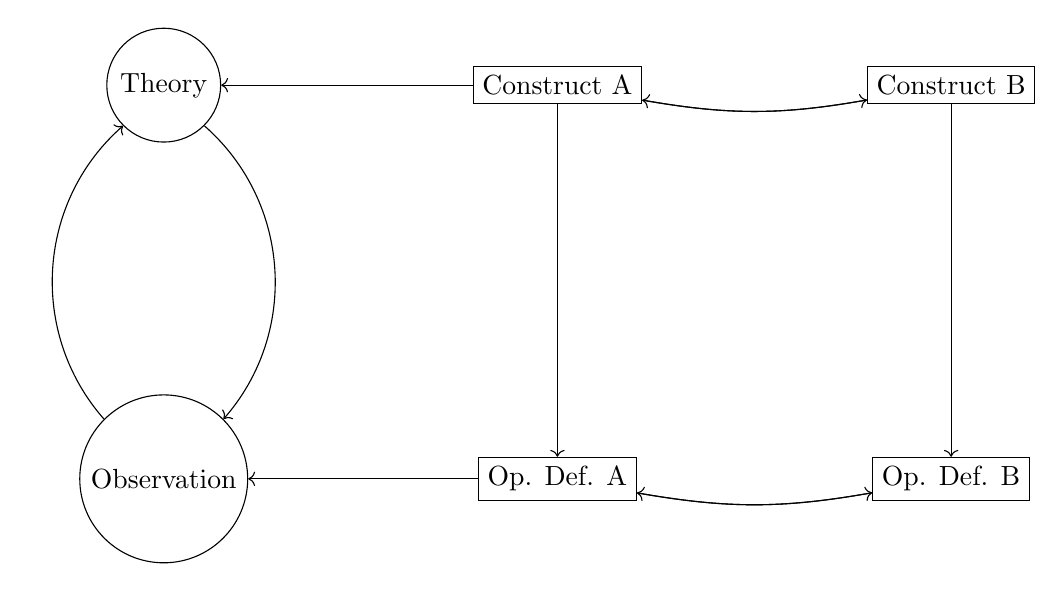
\begin{tikzpicture}[node distance=5cm, auto]
    \tikzset{main node/.style={circle,draw,minimum size=1cm,inner sep=0pt}}
    % Nodes
    \node (theory) [draw, circle] {Theory};
    \node (observation) [below of=theory, draw, circle] {Observation};

    \node (constructA) [right of=theory, draw] {Construct A};
    \node (constructB) [right of=constructA, draw] {Construct B};

    \node (odA) [below of=constructA, draw] {Op. Def. A};
    \node (odB) [below of=constructB, draw] {Op. Def. B};
    
    
    % Arrows
    \draw [->, bend left=45] (theory) to (observation);
    \draw [->, bend left=45] (observation) to (theory);
    \draw [->, left] (constructA) to (theory);
    \draw [->, left] (odA) to (observation);
    \draw [->, bend right=10] (constructA) to (constructB);
    \draw [->, bend left=10] (constructB) to (constructA);
    \draw [->] (constructA) to (odA);
    \draw [->] (constructB) to (odB);
    \draw [->, bend right=10] (odA) to (odB);
    \draw [->, bend left=10] (odB) to (odA);
\end{tikzpicture}
\end{center}

\textit{Operational Definition A, \& B then lead to ...}

\begin{center}
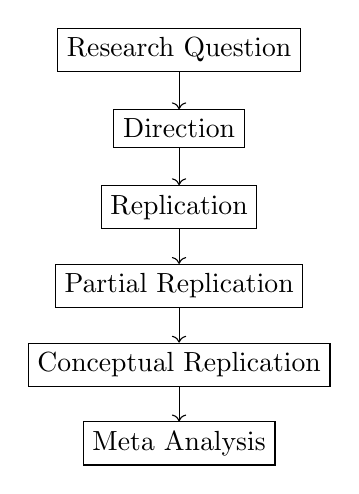
\begin{tikzpicture}
    \tikzset{main node/.style={circle,draw,minimum size=1cm,inner sep=0pt}}
    % Nodes
    \node (RQ) [draw] {Research Question};
    \node (direction) [below of=RQ, draw] {Direction};
    \node (replication) [below of=direction, draw] {Replication};
    \node (part_rep) [below of=replication, draw] {Partial Replication};
    \node (con_rep) [below of=part_rep, draw] {Conceptual Replication};
    \node (meta_analysis) [below of=con_rep, draw] {Meta Analysis};

    % Arrows
    \draw [->] (RQ) to (direction);
    \draw [->] (direction) to (replication);
    \draw [->] (replication) to (part_rep);
    \draw [->] (part_rep) to (con_rep);
    \draw [->] (con_rep) to (meta_analysis);
\end{tikzpicture}
\end{center}

\section{Type of Data}
\begin{itemize}
    \item \textbf{Data:} Output of operational definition.
    \begin{itemize}
        \item Measures; something you will most likely get numbers out of
        \begin{itemize}
            \item Quantitative = Numbers. It's only good if you know what you're looking for in your construct. 
            \item Qualitative = Not Numbers. It is measurable. If you don't feel sure of all of the aspects of your construct.
            \item Mixed Model/Diagram
        \end{itemize}
        \item Manipulation - assign an operational definition to some participants vs. a control group. $\leftarrow$ (Another way to get an operational definition).
        \begin{itemize}
            \item Random
            \item Naturally occurring groups
        \end{itemize}
    \end{itemize}
\end{itemize}

\section{Types of Design}
\begin{itemize}
    \item \textbf{Qualitative Data $\rightarrow$ Qualitative Study:} Going to have research questions. 
    \item \textbf{Quantitiative Data:} Often times discrete and continuous. 
    \begin{itemize}
        \item Discrete
        \item Continuous 
        \begin{itemize}
            \item Exponentially related
            \item Operational Definition = Correlational
        \end{itemize}
    \end{itemize}
    \begin{itemize}
        \item True Experiment - Random Assignment 
        \item Quasi Experiment - Naturally occurring groups
    \end{itemize}
\end{itemize}

\section{Hypothesis Testing}
\begin{itemize}
    \item \textbf{Null Hypothesis}
    \begin{itemize}
        \item $H_0$ $\rightarrow$ no difference/no effect
        \item Experiential(Research Hypothesis) $H_1$ $\rightarrow$ difference is there 
    \end{itemize}
    \item \textbf{Effect Size}
\end{itemize}

\section{Reliability (of studies)}
\begin{itemize}
    \item People can replicate a study. (Replication)
    \item Partial replication. (conceptual replication - not exactly the same sample/outcome measure but lead to similar results)
    \item Meta-analysis. (determines effect size)
\end{itemize}

\section{Validity (of studies)}
\begin{itemize}
    \item Internal Validity - Based on how the study was done, how can we assume that A caused something in B. (How much can we assume this is correct.) 
    \item External Validity - Concerned about how representative our sample is in typical people. 
\end{itemize}

\begin{center}
    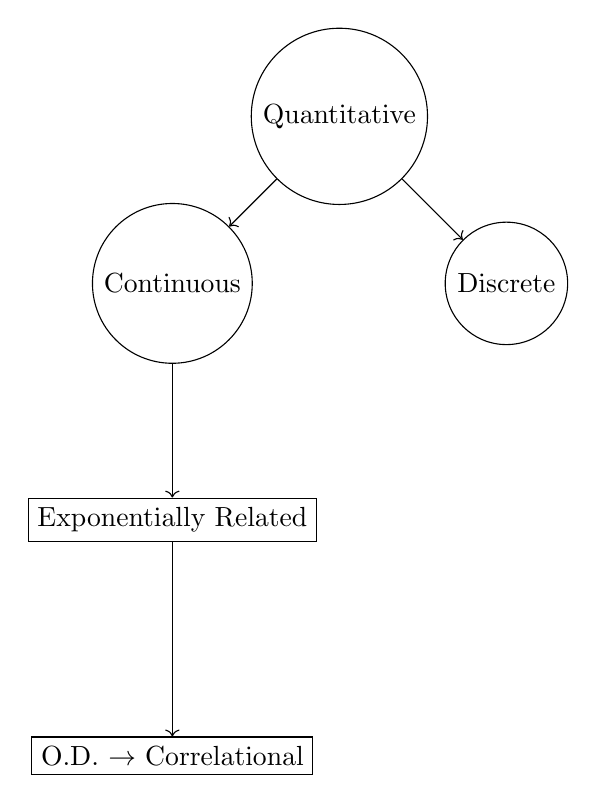
\begin{tikzpicture}[node distance = 3cm, auto]
        \tikzset{main node/.style={circle,draw,minimum size=1cm,inner sep=0pt}}
        
        % Nodes
        \node (quantitative) [draw, circle] {Quantitative};
        \node (continuous) [below left of=quantitative, draw, circle] {Continuous};
        \node (discrete) [below right of=quantitative, draw, circle] {Discrete};
        \node (expo_related) [below of=continuous, draw] {Exponentially Related};
        \node (od_corre) [below of=expo_related, draw] {O.D. $\rightarrow$ Correlational};

        % Arrows
        \draw [->] (quantitative) to (continuous);
        \draw [->] (quantitative) to (discrete);
        \draw [->] (continuous) to (expo_related);
        \draw [->] (expo_related) to (od_corre);
    \end{tikzpicture}
\end{center}

\chapter{Exam 2 Content}

\section{Review Day}

\subsection{Topics}

\subsubsection{Reliability and Validity}
(NOTE: Some more written notes in journal [at 9-19-24])
\begin{itemize}
    \item Reliability = Repeatable measures.
        \begin{itemize}
            \item Ex. Test-Retest Reliability (This only applies to things that should be stable; nothing that is fluctuating.) 
            \item Ex. Interrater Reliability (Reliability over people, not the measure of people but the people doing the measures.) 
            \item Ex. Internal Consistency (This happens when all the items are from the same category. Otherwise, It would be an unfair test.)
        \end{itemize}
    \item Validity = Complex reality vs interpretation. (Is it what it says it is?) 
        \begin{itemize}
            \item Ex. Face Validity - Does it look right? Important when people need to accept your measures. (Flawed)
            \item Ex. Content Validity (Asking experts how valuable the content is.)  
            \item Ex. Criterion Validity (How useful is the measure. How does it predict something that it should predict. i.e., how well does your SAT score predict how well you will do in college?) 
            \item Ex. Convergent and Discriminant Validity (Your measure correlates with things it should correlate with and does not correlate with things that it shouldn't.) 
        \end{itemize}
    \item Note: You can't measure everything $\rightarrow$ sample of items  
    \item Note: Reliability is necessary, but not sufficient, for validity.    
    \item Face validity and content validity are based on people's judgment. 
\end{itemize}

\subsubsection{Popular Press vs. Scholarly Writing}
(NOTE - Some more written notes in journal [at 9-24-24]) 
\begin{itemize}
    \item Goals - 
    \begin{itemize}
        \item Clicks Likes, readers vs. explain theory testing (what's going on)
        \item News
        \item Standards of evidence are different. 
        \item Quotes in the news vs. quotes in scholarly articles.
        \item An angle or hook vs. theory evaluation. 
        \item Bad Science Reporting
        \item Key points vs. Complexity
        \item Editorial vs. Peer Review
        \item Reading and Evaluating Peer-Reviewed Empirical Articles
        \item The format/structure of both is almost the same. 
        \begin{itemize}
            \item Abstract - Tells what we did, why we did it, what we found and what it means. 
            \item (Introduction) Hypothesis - Merging the theory and constructs with how they're defined.
            \item Methods - Participants, Materials (or measures). Finally, the procedure (very narrow section). 
            \item Results - The findings.
            \item Discussion - In the first few paragraphs, the researcher will recap the results section and discuss how the findings support or don't support the theory. Finally, it gives a broader picture and limitations. Also, state how more research is needed or future work. 
        \end{itemize}
    \end{itemize}
\end{itemize}

\subsubsection{How to find these things?}
\begin{itemize}
    \item PsycINFO - Advanced Search (KW = Keywords (Constructs that are in the paper); use check-boxes for "peer-reviewed" and "empirical study." 
    \item Google Scholar (Do not pay for articles - find them from the CU library).
\end{itemize}

\subsubsection{How to not write like a student}
\begin{itemize}
    \item Don't organize by paper; organize by ideas! 
    \item Find "citable bricks" in the description of hypothesis, study, and findings (direct observations reported) 
\end{itemize}

\subsubsection{Statistics (and research design)}
\begin{itemize}
    \item Type of Data: Qualitative Data and Quantitative Data
    \item Quantitative Data 
    \begin{itemize}
        \item Write the definition here
    \end{itemize}
    \item Qualitative Data 
    \begin{itemize}
        \item Write the definition here
    \end{itemize}
    \item Types of Design: Correlational, Experimental, Quasi-Experimental. 
    \item Correlational
    \begin{itemize}
        \item Write the definition here
    \end{itemize}
    \item Experimental 
    \begin{itemize}
        \item Write the definition here
    \end{itemize}
    \item Quasi-Experimental 
    \begin{itemize}
        \item Write the definition here
    \end{itemize}
\end{itemize}

\subsubsection{Hypothesis Testing vs Research Questions}
\begin{itemize}
    \item Null Hypothesis
    \item Effect Size
    \item Reliability (of studies): Replication (how repeatable findings are). 
    \item Validity (of studies): Internal vs. External Validity.
\end{itemize}

\subsubsection{Careers with a Bachelor's Degree in Psychology}

\begin{itemize}
    \item Most Psych majors (over half) don't go on to graduate school.
    \item What careers can you have with a BA or BS? 
    \begin{itemize}
        \item Social Services
        \item Human Resources
        \item Data Analysis and Interpretation 
        \item Sales
        \item Education 
        \item Writing
    \end{itemize}
\end{itemize}

\subsubsection{Other}

\begin{itemize}
    \item Look at graduate school notes.
\end{itemize}

\chapter{Exam 3 Content}

\section{10-24-24}

\subsection{Topics}

\subsubsection{Ed Diener}
A happiness expert using framing.
\begin{itemize}
 \item Know what kinds of things that made people happy 
\end{itemize}

\subsubsection{Can vs. Should}

\begin{itemize}
    \item Consideration 1: Time in major.
    \item Consideration 2: Enjoyment of the KSAs of the Major
    \begin{itemize}
        \item End User Information 
        \item Major level KSAs
        \item Empathy
        \item Objectivity
        \item Tolerance for Ambiguity 
        \begin{itemize}
            \item Error is everywhere for most people most of the time.
        \end{itemize}
        \item Comfort with Multiple Levels of Analysis
        \item Liking to Learn
        \item Precise Language
        \item Statistics and Numbers
    \end{itemize}
    \item Consideration 3a: Career Prospects
    \begin{itemize}
        \item Graduate school? 
        \item Major +
    \end{itemize}
    \item Consideration 3b: Day-to-Day Career Considerations
    \begin{itemize}
        \item Pay (Individual question)
        \item Hours. Also how are they arranged and how much freedom do you have over it? 
        \item Duties and Responsibilities
        \item Other working conditions
    \end{itemize}
\end{itemize}

\subsubsection{Suggestions}
\begin{itemize}
    \item Suggestion 1: Time Perspective
    \item Suggestion 2: Authenticity \& Courageous
    \item Suggestion 3: Be Good to the Future You
    \item Suggestion 4: Be Open to Change
    \item Suggestion 5: Time-Related Biases. 
    \begin{itemize}
        \item Affective Forecasting
        \item Hindsight Bias 
    \end{itemize}
    \item Suggestion 6: Keep Notes
\end{itemize}

\subsubsection{Questions for Consideration}

\sectionquestion{For Consideration 1}{Do you have the time to complete the major? (Do you want to take that long?)}

\sectionquestion{For Consideration 2}{Can you think like a psychology major? Do you enjoy thinking that way?}

\sectionquestion{For Consideration 3a}{Are you willing and able to do the work needed for a career as a psychology major? Would you enjoy it?}

\sectionquestion{For Consideration 3b}{Can you do the day-to-day work in that career? Would you want to?}

\section{10-29-24}
\subsection{Progression through Undergraduate Degree}

\section{10-31-24}
\subsection{Working on Career Plans}

\section{11-7-24}
\subsection{Graduate School Presentation}
\subsection{Notes}
All of the programs presented contain research methods. 
All of the other programs within psychology will contain research methods; they share a common feature: looking at analyzing behavior at the level of the individual.

\subsubsection{KSAs, Competencies, and You!}

\textbf{KSA's:} 

\begin{itemize}
    \item K = Knowledge. What body of information will help you do a particular kind of job or get you into a particular grad program? i.e., basic knowledge in statistics, psychology in health, or other areas of psychology. 
    \item S = Skills. Ways you learn to handle or manipulate things, learnable things, or how to do things. 
    \item A = Abilities. Some basic thing about you that makes something easier for you. i.e., good at thinking numerically.
\end{itemize}

\noindent \textbf{Competencies = Ks + Ss + As}
\newline
Can you explain what you need to know for a job and how you need to know how to do that? 
\begin{itemize}
    \item Overt Competencies. 
    \begin{itemize}
        \item Particularly true when you are thinking about planning your coursework.
        \item Course Objectives and learning outcomes.
    \end{itemize}
    \item Covert Competencies.
    \begin{itemize}
        \item Think about how you learn about how you've learned the overt competencies!
        \item These are critical thinking and problem-solving, oral and written communication, teamwork and collaboration, digital technology, leadership, professional/work ethics, career management, and global and intercultural fluency.
    \end{itemize}
    \item Titles of Courses? $\rightarrow$ What you are learning and what you want to learn.
    \item Places to look: Course Catalog, Syllabus Repository.
\end{itemize}

\textbf{Competencies for Psych majors}
\begin{itemize}
    \item Knowledge base in psychology.
    \item Scientific inquiry and critical thinking.
    \item Ethical and social responsibility in a diverse world.
    \item Communication.
    \item Professional Developmentedswf
\end{itemize}

\section{11-14-25}

\subsection{Competencies From Extra Curriculars and What do you want to do at work? }
 
\sectiondefinition{Extracurricular}{Any activity that is not required for school and is not graded}

\sectionexample{Extracurriculars}
{
    \begin{itemize}
        \item Jobs
        \item Volunteer Work
        \item Clubs
        \item Anything at Tiger Prowl
        \item Community Groups
        \item Internships
        \item Study Abroad
        \item Other!
    \end{itemize}
}

\sectionquestion{Random}{What do you want to do at work?}

\sectionexample{O*Net - Where to find what to do.}
{
\begin{itemize}
    \item Tasks Tech Skills
    \item Work Activities 
    \item Work Context
\end{itemize}
}

\chapter{Final Exam}

\section{Topics}
Consilience is a stretched out Biopsychosocial model \\
Psychology: The scientific study of people and other animals (beings?) at the individual level. \\ 
History of Psychology: Not no final \\ 
fundamental processes : Why do these things happen? Is what we are interested in. 
\begin{itemize}
    \item Psych classes like sensation perception etc.
\end{itemize}
We are also interested in applications to various settings. How we can make peoples lives better or change something somehow. Or applying something to something specific. 
\begin{itemize}
    \item Abnormal psych
    \item IO psych 
    \item Human factors psychology 
\end{itemize}

\subsection{The Science Cycle}
Theory which is the relationship between two constructs. \\ 
This then goes into operational definition of constructs. This includes making a hypothesis which is making a relationship with two or more operational definitions. \\
This then goes into making observations \\ 
Then this goes into results and then back into theory. \\

Exam will question theory, construct, and measure. \\ 

\subsubsection{Manipulation:} 
How can we change the amount of ?
\subsubsection{Measurement:}
How do we know if there is more or less of ? 

Note: both measures and manipulations of a construct are operational definitions. \\ 

Theory $\rightarrow$ Hypothesis (operational definition 1 and operational definition 2 
) $\rightarrow$ Observations $\rightarrow$ Results $\rightarrow$ data analysis (sees how the data
relates to the theory) $\rightarrow$ theory \\

Note: the two primary ways we can analyze data are with 
null hypothesis testing and effect size. \\ 

Observed score = true score + error \\ 
How much of this scores operational definition reflects the construct. If a measures 
score is not good, then it must have a lot of error and its validity is not great. \\
Reliability and validity in measurement of individuals.

Reliability - can you do it over again and get the same answer? Over tine, over observers, and over items (interested in) 

Test - retest reliability \\ 
Interrater reliability (over observers i.e., if a teacher graded something and a TA graded it too and you get the same grade) \\ 
Internal consistency (over items are the items all corrallary to one another) \\ 

Validity? = is it what it says it is? How much does the measure relate to the actual construct? \\ 
Face validity (not a good argument in actual validity) \\
Content validity = if experts agree that you have covered the major basis \\ 
Criterion validity = How much does a thing report how good it is via testing \\
Convergent and discriminant validity = how much it correlates how much it doesn't. \\
Reliability is necessary, but not sufficient for validity. \\ 
Construct validity = does the operational definition measure the construct? \\
Popular press vs scholarly writing differ by goals, evidence, use of quotes, type of review. \\ 
editorial review vs peer reviewer \\ 
Citable bricks \\
\begin{itemize}
    \item Abstract
    \item Introduction 
    \item Results 
    \item Discussion
\end{itemize}

\begin{itemize}
    \item types of data: 
    \begin{itemize}
        \item Life data 
        \item Observers - Interrater reliability. Two types of observers: People that are experts in the person, and people who 
        are experts in whatever that construct is 
        \item Test data - super standardized and reliable
        \item self report - survey data on what the person says they are  
    \end{itemize}
    \item types of design: 
    \item Hypothesis testing
    \begin{itemize}
        \item Null hypothesis
        \item Effect size 
        \item Reliability of studies 
        \item validity of studies 
    \end{itemize}
\end{itemize}

\section{More Topics}

Note: Cumulative final exam: Wed, 12/11 8 - 10:30 am fifty multiple choice questions.

Correlational design - both operational definitions are just measured 
and not manipulated. \\
Experimental design - one operational definition is manipulated and the other is 
measured. \\

Theory and hypothesis are covered by the intro. Hypothesis then to observations are covered by the methods.
Observations and then to data analyzing are covered by results. Data analyzing to theory 
are covered by the discussion. \\ 

\chapter{References}
This is a reference to a source \cite{example}.

\bibliographystyle{plain}
\bibliography{references}


\end{document}